\chapter{树}

\section{AVL树}

\subsection{AVL树}

AVL树的命名是取自两位发明者的首字母G. M. Adelson-Velsky和E. M. Landis,AVL树也称为平衡二叉树。 \\

AVL树能够调整自身的平衡性,AVL树遵循高度平衡,任何结点的两个子树高度差不会超过1。 \\

对于AVL树的每一个结点,平衡因子(balance factor)是它左子树高度和右子树高度的差值。只有当二叉树所有结点的平衡因子都是-1、0、1这三个值时,这棵树才是一个合格的AVL树。 \\

\begin{figure}[H]
	\centering
	\begin{tikzpicture}[
			level distance=1.5cm,
			level 1/.style={sibling distance=4cm},
			level 2/.style={sibling distance=2cm},
			level 3/.style={sibling distance=1cm}
		]
		\node[circle,draw] {A}
		child {
				node[circle,draw] {B}
				child {
						node[circle,draw] {D}
						child[missing] {}
						child {node[circle,draw] {G}}
					}
				child {node[circle,draw] {E}}
			}
		child {
				node[circle,draw] {C}
				child[missing] {}
				child {node[circle,draw] {F}}
			};
	\end{tikzpicture}
	\caption{AVL树}
\end{figure}

\begin{figure}[H]
	\centering
	\begin{tikzpicture}[
			level distance=1.5cm,
			level 1/.style={sibling distance=4cm},
			level 2/.style={sibling distance=2cm},
			level 3/.style={sibling distance=1cm}
		]
		\node[circle,draw] {A}
		child {
				node[circle,draw] {B}
				child {
						node[circle,draw] {D}
						child[missing] {}
						child {node[circle,draw] {G}}
					}
				child {node[circle,draw] {E}}
			}
		child {node[circle,draw] {C}};
	\end{tikzpicture}
	\caption{非AVL树}
\end{figure}

\begin{figure}[H]
	\centering
	\begin{tikzpicture}[
			level distance=1.5cm,
			level 1/.style={sibling distance=4cm},
			level 2/.style={sibling distance=2cm},
			level 3/.style={sibling distance=1cm}
		]
		\node[circle,draw] {A}
		child {
				node[circle,draw] {B}
				child {
						node[circle,draw] {D}
						child {node[circle,draw] {F}}
						child[missing] {}
					}
				child[missing] {}
			}
		child {
				node[circle,draw] {C}
				child[missing] {}
				child {
						node[circle,draw] {E}
						child[missing] {}
						child {node[circle,draw] {G}}
					}
			};
	\end{tikzpicture}
	\caption{非AVL树}
\end{figure}

\subsection{失衡调整}

当AVL树插入或删除结点时,平衡有可能被打破。 \\

\begin{figure}[H]
	\centering
	\begin{tikzpicture}[
			level distance=1.5cm,
			level 1/.style={sibling distance=4cm},
			level 2/.style={sibling distance=2cm},
			level 3/.style={sibling distance=1cm}
		]
		\node[circle,draw] {A}
		child {
				node[circle,draw] {B}
				child {
						node[circle,draw] {D}
						child {node[circle,draw] {\textcolor{red}{G}}}
						child[missing] {}
					}
				child[missing] {}
			}
		child {
				node[circle,draw] {C}
				child {node[circle,draw] {E}}
				child {node[circle,draw] {F}}
			};
	\end{tikzpicture}
	\caption{失衡}
\end{figure}

通过对AVL树进行左旋转、右旋转的操作,就能使其重新恢复平衡。

\subsubsection{左旋转}

逆时针旋转AVL树的两个结点X和Y,使得父结点被自己的右孩子取代,而自己成为左孩子。

\begin{figure}[H]
	\centering
	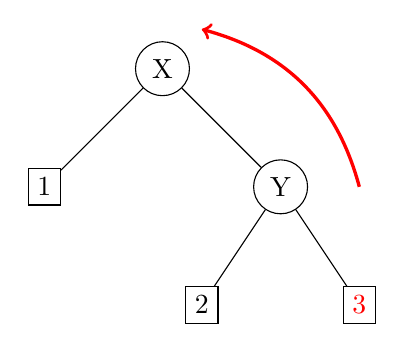
\begin{tikzpicture}[
			level distance=1.5cm,
			level 1/.style={sibling distance=3cm},
			level 2/.style={sibling distance=2cm},
			level 3/.style={sibling distance=1cm}
		]
		\node[circle,draw] {X}
		child {node[rectangle,draw] {1}}
		child {
				node[circle,draw] {Y}
				child {node[rectangle,draw] {2}}
				child {node[rectangle,draw] {\textcolor{red}{3}}}
			};

		\draw[->, very thick, red] (2.5,-1.5) to[bend right] (0.5,0.5);
	\end{tikzpicture}
	\caption{左旋转(前)}
\end{figure}

\begin{figure}[H]
	\centering
	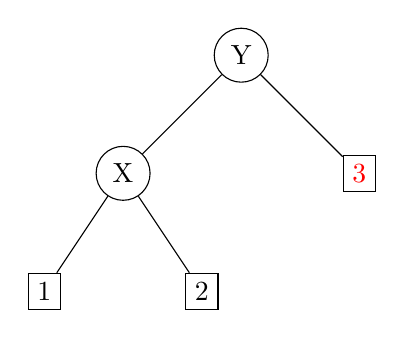
\begin{tikzpicture}[
			level distance=1.5cm,
			level 1/.style={sibling distance=3cm},
			level 2/.style={sibling distance=2cm},
			level 3/.style={sibling distance=1cm}
		]
		\node[circle,draw] {Y}
		child {
				node[circle,draw] {X}
				child {node[rectangle,draw] {1}}
				child {node[rectangle,draw] {2}}
			}
		child {
				node[rectangle,draw] {\textcolor{red}{3}}
			};
	\end{tikzpicture}
	\caption{左旋转(后)}
\end{figure}

\subsubsection{右旋转}

顺时针旋转AVL树的两个结点X和Y,使得父结点被自己的左孩子取代,而自己成为右孩子。

\begin{figure}[H]
	\centering
	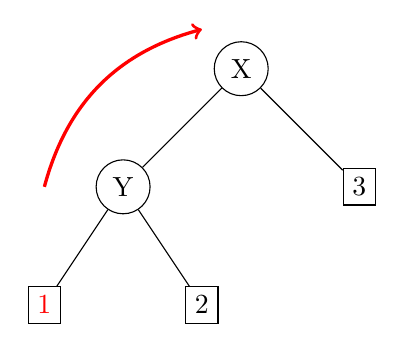
\begin{tikzpicture}[
			level distance=1.5cm,
			level 1/.style={sibling distance=3cm},
			level 2/.style={sibling distance=2cm},
			level 3/.style={sibling distance=1cm}
		]
		\node[circle,draw] {X}
		child {
				node[circle,draw] {Y}
				child {node[rectangle,draw] {\textcolor{red}{1}}}
				child {node[rectangle,draw] {2}}
			}
		child {node[rectangle,draw] {3}};

		\draw[->, very thick, red] (-2.5,-1.5) to[bend left] (-0.5,0.5);
	\end{tikzpicture}
	\caption{右旋转(前)}
\end{figure}

\begin{figure}[H]
	\centering
	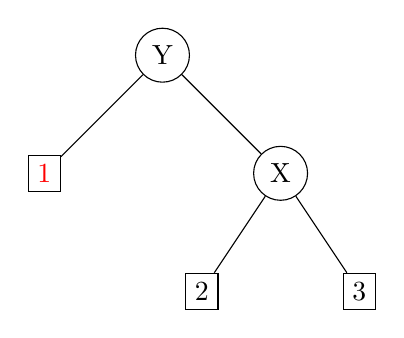
\begin{tikzpicture}[
			level distance=1.5cm,
			level 1/.style={sibling distance=3cm},
			level 2/.style={sibling distance=2cm},
			level 3/.style={sibling distance=1cm}
		]
		\node[circle,draw] {Y}
		child {node[rectangle,draw] {\textcolor{red}{1}}}
		child {
				node[circle,draw] {X}
				child {node[rectangle,draw] {2}}
				child {node[rectangle,draw] {3}}
			};
	\end{tikzpicture}
	\caption{右旋转(后)}
\end{figure}

AVL树的失衡调整可以分为四种情况:

\subsubsection{左左局面(LL):右旋转}

\begin{figure}[H]
	\centering
	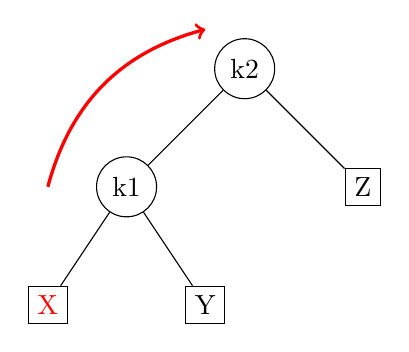
\begin{tikzpicture}[
			level distance=1.5cm,
			level 1/.style={sibling distance=3cm},
			level 2/.style={sibling distance=2cm},
			level 3/.style={sibling distance=1cm}
		]
		\node[circle,draw] {k2}
		child {
				node[circle,draw] {k1}
				child {node[rectangle,draw] {\textcolor{red}{X}}}
				child {node[rectangle,draw] {Y}}
			}
		child {node[rectangle,draw] {Z}};

		\draw[->, very thick, red] (-2.5,-1.5) to[bend left] (-0.5,0.5);
	\end{tikzpicture}
	\caption{左左局面}
\end{figure}

\begin{figure}[H]
	\centering
	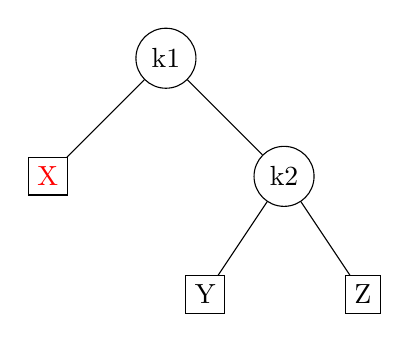
\begin{tikzpicture}[
			level distance=1.5cm,
			level 1/.style={sibling distance=3cm},
			level 2/.style={sibling distance=2cm},
			level 3/.style={sibling distance=1cm}
		]
		\node[circle,draw] {k1}
		child {node[rectangle,draw] {\textcolor{red}{X}}}
		child {
				node[circle,draw] {k2}
				child {node[rectangle,draw] {Y}}
				child {node[rectangle,draw] {Z}}
			};
	\end{tikzpicture}
	\caption{右旋转}
\end{figure}

\mybox{LL旋转}

\begin{lstlisting}[language=C]
static AVLNode* LLRotation(AVLTree *k2) {
    AVLTree *k1 = k2->left;
    k2->left = k1->right;
    k1->right = k2;
    
    k2->height = max(height(k2->left), height(k2->right)) + 1;
    k1->height = max(height(k1->left), k2->height) + 1;
    return k1;
}
\end{lstlisting}

\subsubsection{右右局面(RR):左旋转}

\begin{figure}[H]
	\centering
	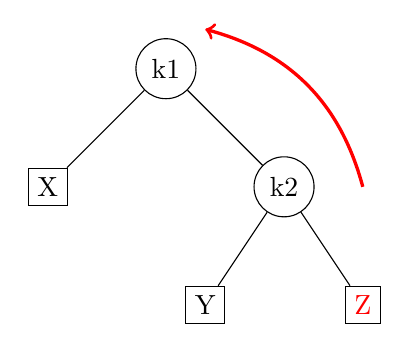
\begin{tikzpicture}[
			level distance=1.5cm,
			level 1/.style={sibling distance=3cm},
			level 2/.style={sibling distance=2cm},
			level 3/.style={sibling distance=1cm}
		]
		\node[circle,draw] {k1}
		child {node[rectangle,draw] {X}}
		child {
				node[circle,draw] {k2}
				child {node[rectangle,draw] {Y}}
				child {node[rectangle,draw] {\textcolor{red}{Z}}}
			};

		\draw[->, very thick, red] (2.5,-1.5) to[bend right] (0.5,0.5);
	\end{tikzpicture}
	\caption{右右局面}
\end{figure}

\begin{figure}[H]
	\centering
	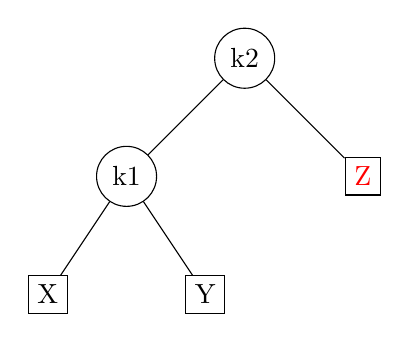
\begin{tikzpicture}[
			level distance=1.5cm,
			level 1/.style={sibling distance=3cm},
			level 2/.style={sibling distance=2cm},
			level 3/.style={sibling distance=1cm}
		]
		\node[circle,draw] {k2}
		child {
				node[circle,draw] {k1}
				child {node[rectangle,draw] {X}}
				child {node[rectangle,draw] {Y}}
			}
		child {node[rectangle,draw] {\textcolor{red}{Z}}};
	\end{tikzpicture}
	\caption{左旋转}
\end{figure}

\mybox{RR旋转}

\begin{lstlisting}[language=C]
static AVLNode* RRRotation(AVLTree *k1) {
    AVLTree *k2 = k1->right;
    k1->right = k2->left;
    k2->left = k1;

    k1->height = max(height(k1->left), height(k1->right)) + 1;
    k2->height = max(k1->height, height(k2->right)) + 1;
    return k2;
}
\end{lstlisting}

\subsubsection{左右局面(LR):先左旋转、再右旋转}

\begin{figure}[H]
	\centering
	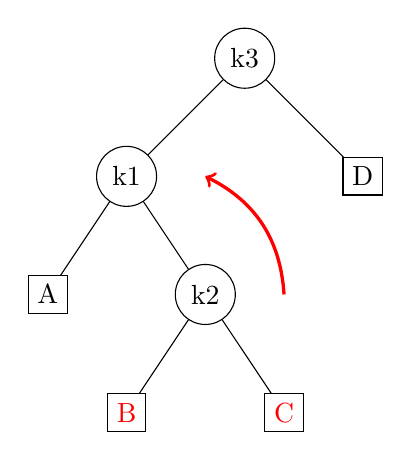
\begin{tikzpicture}[
			level distance=1.5cm,
			level 1/.style={sibling distance=3cm},
			level 2/.style={sibling distance=2cm},
			level 3/.style={sibling distance=2cm}
		]
		\node[circle,draw] {k3}
		child {
				node[circle,draw] {k1}
				child {node[rectangle,draw] {A}}
				child {
						node[circle,draw] {k2}
						child {node[rectangle,draw] {\textcolor{red}{B}}}
						child {node[rectangle,draw] {\textcolor{red}{C}}}
					}
			}
		child {node[rectangle,draw] {D}};

		\draw[->, very thick, red] (0.5,-3) to[bend right] (-0.5,-1.5);
	\end{tikzpicture}
	\caption{左右局面}
\end{figure}

\begin{figure}[H]
	\centering
	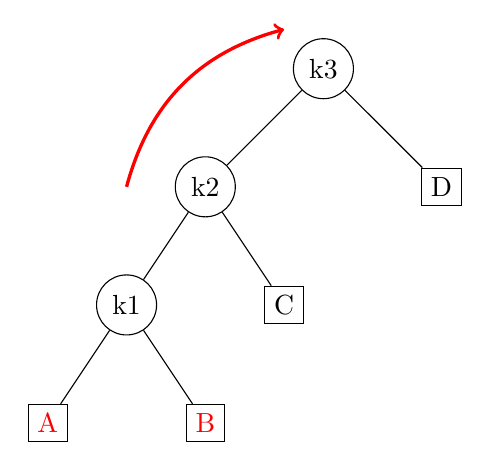
\begin{tikzpicture}[
			level distance=1.5cm,
			level 1/.style={sibling distance=3cm},
			level 2/.style={sibling distance=2cm},
			level 3/.style={sibling distance=2cm}
		]
		\node[circle,draw] {k3}
		child {
				node[circle,draw] {k2}
				child {
						node[circle,draw] {k1}
						child {node[rectangle,draw] {\textcolor{red}{A}}}
						child {node[rectangle,draw] {\textcolor{red}{B}}}
					}
				child {node[rectangle,draw] {C}}
			}
		child {node[rectangle,draw] {D}};

		\draw[->, very thick, red] (-2.5,-1.5) to[bend left] (-0.5,0.5);
	\end{tikzpicture}
	\caption{左旋转}
\end{figure}

\begin{figure}[H]
	\centering
	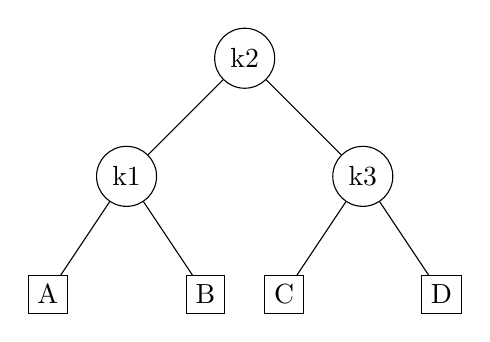
\begin{tikzpicture}[
			level distance=1.5cm,
			level 1/.style={sibling distance=3cm},
			level 2/.style={sibling distance=2cm},
			level 3/.style={sibling distance=2cm}
		]
		\node[circle,draw] {k2}
		child {
				node[circle,draw] {k1}
				child {node[rectangle,draw] {A}}
				child {node[rectangle,draw] {B}}
			}
		child {
				node[circle,draw] {k3}
				child {node[rectangle,draw] {C}}
				child {node[rectangle,draw] {D}}
			};
	\end{tikzpicture}
	\caption{右旋转}
\end{figure}

\mybox{LR旋转}

\begin{lstlisting}[language=C]
static AVLNode* LRRotation(AVLTree *k3) {
    k3->left = RRRotation(k3->left);
    return LLRotation(k3);
}
\end{lstlisting}

\subsubsection{右左局面(RL):先右旋转、再左旋转}

\begin{figure}[H]
	\centering
	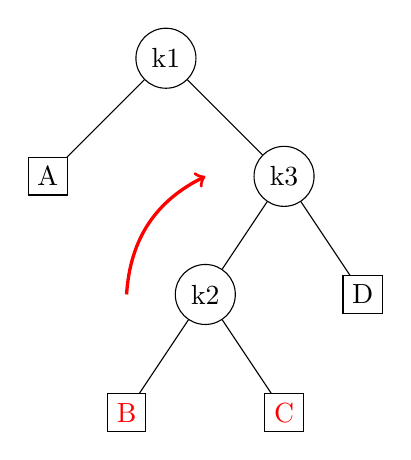
\begin{tikzpicture}[
			level distance=1.5cm,
			level 1/.style={sibling distance=3cm},
			level 2/.style={sibling distance=2cm},
			level 3/.style={sibling distance=2cm}
		]
		\node[circle,draw] {k1}
		child {node[rectangle,draw] {A}}
		child {
				node[circle,draw] {k3}
				child {
						node[circle,draw] {k2}
						child {node[rectangle,draw] {\textcolor{red}{B}}}
						child {node[rectangle,draw] {\textcolor{red}{C}}}
					}
				child {node[rectangle,draw] {D}}
			};

		\draw[->, very thick, red] (-0.5,-3) to[bend left] (0.5,-1.5);
	\end{tikzpicture}
	\caption{右左局面}
\end{figure}

\begin{figure}[H]
	\centering
	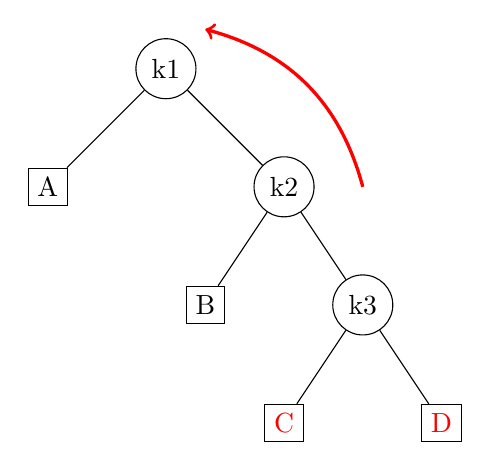
\begin{tikzpicture}[
			level distance=1.5cm,
			level 1/.style={sibling distance=3cm},
			level 2/.style={sibling distance=2cm},
			level 3/.style={sibling distance=2cm}
		]
		\node[circle,draw] {k1}
		child {node[rectangle,draw] {A}}
		child {
				node[circle,draw] {k2}
				child {node[rectangle,draw] {B}}
				child {
						node[circle,draw] {k3}
						child {node[rectangle,draw] {\textcolor{red}{C}}}
						child {node[rectangle,draw] {\textcolor{red}{D}}}
					}
			};

		\draw[->, very thick, red] (2.5,-1.5) to[bend right] (0.5,0.5);
	\end{tikzpicture}
	\caption{右旋转}
\end{figure}

\begin{figure}[H]
	\centering
	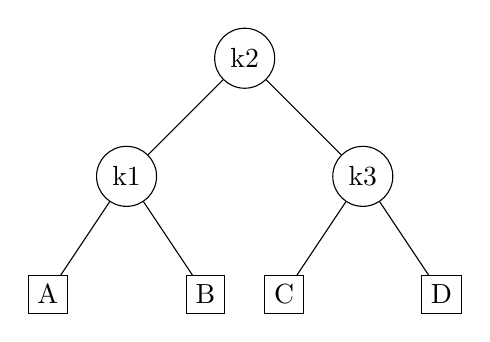
\begin{tikzpicture}[
			level distance=1.5cm,
			level 1/.style={sibling distance=3cm},
			level 2/.style={sibling distance=2cm},
			level 3/.style={sibling distance=2cm}
		]
		\node[circle,draw] {k2}
		child {
				node[circle,draw] {k1}
				child {node[rectangle,draw] {A}}
				child {node[rectangle,draw] {B}}
			}
		child {
				node[circle,draw] {k3}
				child {node[rectangle,draw] {C}}
				child {node[rectangle,draw] {D}}
			};
	\end{tikzpicture}
	\caption{左旋转}
\end{figure}

\mybox{RL旋转}

\begin{lstlisting}[language=C]
static AVLNode* RLRotation(AVLTree *k1) {
    k1->right = LLRotation(k1->right);
    return RRRotation(k1);
}
\end{lstlisting}

\subsection{插入/删除结点}

例如依次向AVL树添加结点3, 2, 1, 4, 5, 6, 7, 16, 15, 14。

\begin{figure}[H]
	\centering
	\begin{tikzpicture}[
			level distance=1.5cm,
			level 1/.style={sibling distance=3cm},
			level 2/.style={sibling distance=2cm},
			level 3/.style={sibling distance=2cm}
		]
		\node[circle,draw] {3}
		child {
				node[circle,draw] {2}
				child {node[circle,draw] {1}}
				child[missing] {}
			}
		child[missing] {};
	\end{tikzpicture}
	\caption{左左局面:插入3、2、1}
\end{figure}

\begin{figure}[H]
	\centering
	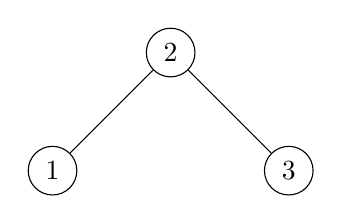
\begin{tikzpicture}[
			level distance=1.5cm,
			level 1/.style={sibling distance=3cm},
			level 2/.style={sibling distance=2cm},
			level 3/.style={sibling distance=2cm}
		]
		\node[circle,draw] {2}
		child {node[circle,draw] {1}}
		child {node[circle,draw] {3}};
	\end{tikzpicture}
	\caption{右旋转}
\end{figure}

\begin{figure}[H]
	\centering
	\begin{tikzpicture}[
			level distance=1.5cm,
			level 1/.style={sibling distance=3cm},
			level 2/.style={sibling distance=2cm},
			level 3/.style={sibling distance=2cm}
		]
		\node[circle,draw] {2}
		child {node[circle,draw] {1}}
		child {
				node[circle,draw] {3}
				child[missing] {}
				child {
						node[circle,draw] {4}
						child[missing] {}
						child {node[circle,draw] {5}}
					}
			};
	\end{tikzpicture}
	\caption{右右局面:插入4、5}
\end{figure}

\begin{figure}[H]
	\centering
	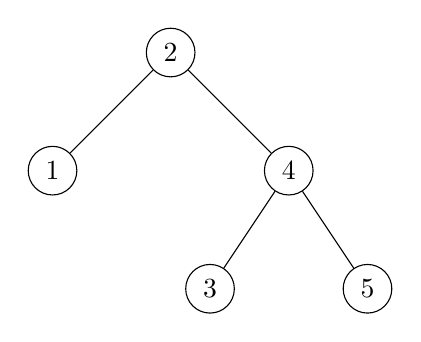
\begin{tikzpicture}[
			level distance=1.5cm,
			level 1/.style={sibling distance=3cm},
			level 2/.style={sibling distance=2cm},
			level 3/.style={sibling distance=2cm}
		]
		\node[circle,draw] {2}
		child {node[circle,draw] {1}}
		child {
				node[circle,draw] {4}
				child {node[circle,draw] {3}}
				child {node[circle,draw] {5}}
			};
	\end{tikzpicture}
	\caption{左旋转}
\end{figure}

\begin{figure}[H]
	\centering
	\begin{tikzpicture}[
			level distance=1.5cm,
			level 1/.style={sibling distance=3cm},
			level 2/.style={sibling distance=2cm},
			level 3/.style={sibling distance=2cm}
		]
		\node[circle,draw] {2}
		child {node[circle,draw] {1}}
		child {
				node[circle,draw] {4}
				child {node[circle,draw] {3}}
				child {
						node[circle,draw] {5}
						child[missing] {}
						child {node[circle,draw] {6}}
					}
			};
	\end{tikzpicture}
	\caption{右右局面:插入6}
\end{figure}

\begin{figure}[H]
	\centering
	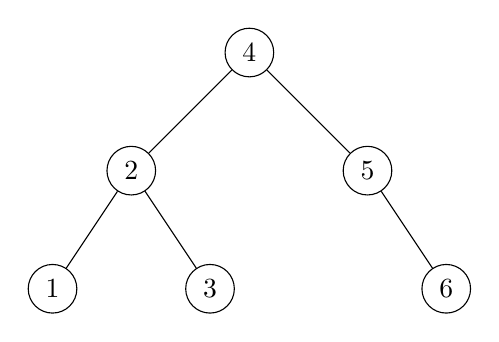
\begin{tikzpicture}[
			level distance=1.5cm,
			level 1/.style={sibling distance=3cm},
			level 2/.style={sibling distance=2cm},
			level 3/.style={sibling distance=2cm}
		]
		\node[circle,draw] {4}
		child {
				node[circle,draw] {2}
				child {node[circle,draw] {1}}
				child {node[circle,draw] {3}}
			}
		child {
				node[circle,draw] {5}
				child[missing] {}
				child {node[circle,draw] {6}}
			};
	\end{tikzpicture}
	\caption{左旋转}
\end{figure}

\begin{figure}[H]
	\centering
	\begin{tikzpicture}[
			level distance=1.5cm,
			level 1/.style={sibling distance=3cm},
			level 2/.style={sibling distance=2cm},
			level 3/.style={sibling distance=2cm}
		]
		\node[circle,draw] {4}
		child {
				node[circle,draw] {2}
				child {node[circle,draw] {1}}
				child {node[circle,draw] {3}}
			}
		child {
				node[circle,draw] {5}
				child[missing] {}
				child {
						node[circle,draw] {6}
						child[missing] {}
						child {node[circle,draw] {7}}
					}
			};
	\end{tikzpicture}
	\caption{右右局面:插入7}
\end{figure}

\begin{figure}[H]
	\centering
	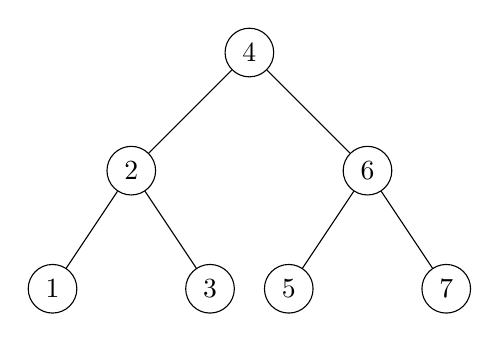
\begin{tikzpicture}[
			level distance=1.5cm,
			level 1/.style={sibling distance=3cm},
			level 2/.style={sibling distance=2cm},
			level 3/.style={sibling distance=2cm}
		]
		\node[circle,draw] {4}
		child {
				node[circle,draw] {2}
				child {node[circle,draw] {1}}
				child {node[circle,draw] {3}}
			}
		child {
				node[circle,draw] {6}
				child {node[circle,draw] {5}}
				child {node[circle,draw] {7}}
			};
	\end{tikzpicture}
	\caption{左旋转}
\end{figure}

\begin{figure}[H]
	\centering
	\begin{tikzpicture}[
			level distance=1.5cm,
			level 1/.style={sibling distance=3cm},
			level 2/.style={sibling distance=2cm},
			level 3/.style={sibling distance=2cm}
		]
		\node[circle,draw] {4}
		child {
				node[circle,draw] {2}
				child {node[circle,draw] {1}}
				child {node[circle,draw] {3}}
			}
		child {
				node[circle,draw] {6}
				child {node[circle,draw] {5}}
				child {
						node[circle,draw] {7}
						child[missing] {}
						child {
								node[circle,draw] {16}
								child {node[circle,draw] {15}}
								child[missing] {}
							}
					}
			};
	\end{tikzpicture}
	\caption{右左局面:插入16、15}
\end{figure}

\begin{figure}[H]
	\centering
	\begin{tikzpicture}[
			level distance=1.5cm,
			level 1/.style={sibling distance=3cm},
			level 2/.style={sibling distance=2cm},
			level 3/.style={sibling distance=2cm}
		]
		\node[circle,draw] {4}
		child {
				node[circle,draw] {2}
				child {node[circle,draw] {1}}
				child {node[circle,draw] {3}}
			}
		child {
				node[circle,draw] {6}
				child {node[circle,draw] {5}}
				child {
						node[circle,draw] {7}
						child[missing] {}
						child {
								node[circle,draw] {15}
								child[missing] {}
								child {node[circle,draw] {16}}
							}
					}
			};
	\end{tikzpicture}
	\caption{右旋转}
\end{figure}

\begin{figure}[H]
	\centering
	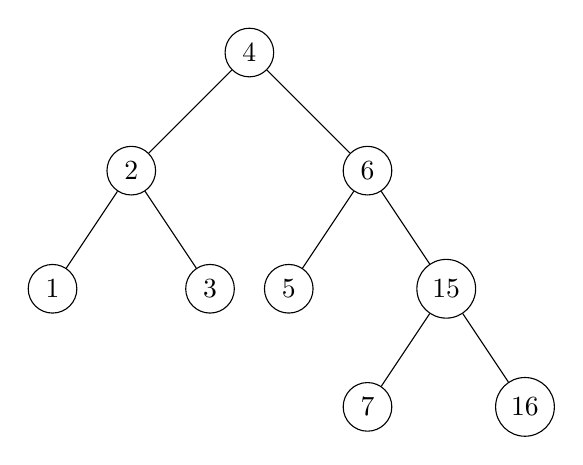
\begin{tikzpicture}[
			level distance=1.5cm,
			level 1/.style={sibling distance=3cm},
			level 2/.style={sibling distance=2cm},
			level 3/.style={sibling distance=2cm}
		]
		\node[circle,draw] {4}
		child {
				node[circle,draw] {2}
				child {node[circle,draw] {1}}
				child {node[circle,draw] {3}}
			}
		child {
				node[circle,draw] {6}
				child {node[circle,draw] {5}}
				child {
						node[circle,draw] {15}
						child {node[circle,draw] {7}}
						child {node[circle,draw] {16}}
					}
			};
	\end{tikzpicture}
	\caption{左旋转}
\end{figure}

\begin{figure}[H]
	\centering
	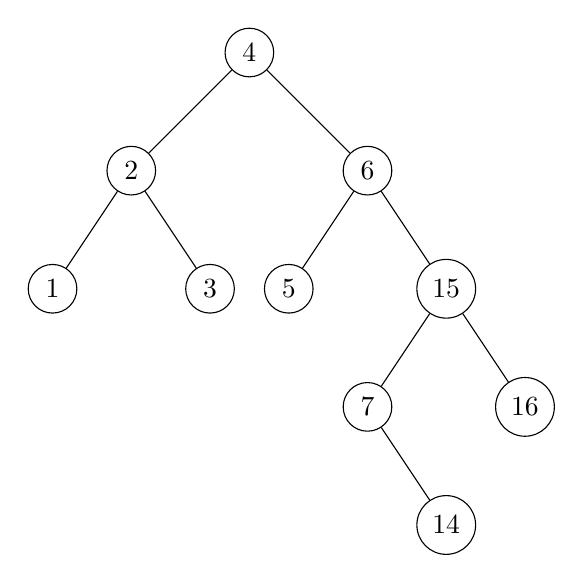
\begin{tikzpicture}[
			level distance=1.5cm,
			level 1/.style={sibling distance=3cm},
			level 2/.style={sibling distance=2cm},
			level 3/.style={sibling distance=2cm}
		]
		\node[circle,draw] {4}
		child {
				node[circle,draw] {2}
				child {node[circle,draw] {1}}
				child {node[circle,draw] {3}}
			}
		child {
				node[circle,draw] {6}
				child {node[circle,draw] {5}}
				child {
						node[circle,draw] {15}
						child {
								node[circle,draw] {7}
								child[missing] {}
								child {node[circle,draw] {14}}
							}
						child {node[circle,draw] {16}}
					}
			};
	\end{tikzpicture}
	\caption{右左局面:插入14}
\end{figure}

\begin{figure}[H]
	\centering
	\begin{tikzpicture}[
			level distance=1.5cm,
			level 1/.style={sibling distance=3cm},
			level 2/.style={sibling distance=2cm},
			level 3/.style={sibling distance=2cm}
		]
		\node[circle,draw] {4}
		child {
				node[circle,draw] {2}
				child {node[circle,draw] {1}}
				child {node[circle,draw] {3}}
			}
		child {
				node[circle,draw] {6}
				child {node[circle,draw] {5}}
				child {
						node[circle,draw] {7}
						child {node[circle,draw] {14}}
						child {
								node[circle,draw] {15}
								child[missing] {}
								child {node[circle,draw] {16}}
							}
					}
			};
	\end{tikzpicture}
	\caption{右旋转}
\end{figure}

\begin{figure}[H]
	\centering
	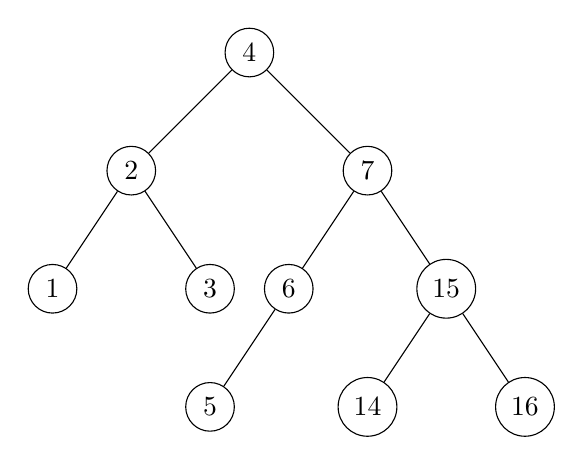
\begin{tikzpicture}[
			level distance=1.5cm,
			level 1/.style={sibling distance=3cm},
			level 2/.style={sibling distance=2cm},
			level 3/.style={sibling distance=2cm}
		]
		\node[circle,draw] {4}
		child {
				node[circle,draw] {2}
				child {node[circle,draw] {1}}
				child {node[circle,draw] {3}}
			}
		child {
				node[circle,draw] {7}
				child {
						node[circle,draw] {6}
						child {node[circle,draw] {5}}
						child[missing] {}
					}
				child {
						node[circle,draw] {15}
						child {node[circle,draw] {14}}
						child {node[circle,draw] {16}}
					}
			};
	\end{tikzpicture}
	\caption{左旋转}
\end{figure}

\mybox{插入结点}

\begin{lstlisting}[language=C]
AVLNode* insert(AVLTree *tree, dataType val) {
    if(!tree) {
        tree = createNode(val, NULL, NULL);
        tree->height = 1;
        return tree;
    }

    if(val < tree->data) {
        tree->left = insert(tree->left, val);
        if(height(tree->left) - height(tree->right) == 2) {
            if(val < tree->left->data) {
                tree = LLRotation(tree);
            } else {
                tree = LRRotation(tree);
            }
        }
    } else {
        tree->right = insert(tree->right, val);
        if(height(tree->right) - height(tree->left) == 2) {
            if(val > tree->right->data) {
                tree = RRRotation(tree);
            } else {
                tree = RLRotation(tree);
            }
        }
    }

    tree->height = max(height(tree->left), height(tree->right)) + 1;
    return tree;
}
\end{lstlisting}

\mybox{删除结点}

\begin{lstlisting}[language=C]
static AVLNode* deleteNode(AVLTree *tree, AVLNode *del) {
    if(!tree || !del) {
        return NULL;
    }

    if(del->data < tree->data) {
        tree->left = deleteNode(tree->left, del);
        if(height(tree->right) - height(tree->left) == 2) {
            AVLNode *rightNode = tree->right;
            if(height(rightNode->left) > height(rightNode->right)) {
                tree = RLRotation(tree);
            } else {
                tree = RRRotation(tree);
            }
        }
    } else if(del->data > tree->data) {
        tree->right = deleteNode(tree->right, del);
        if(height(tree->left) - height(tree->right) == 2) {
            AVLNode *leftNode = tree->left;
            if(height(leftNode->right) > height(leftNode->left)) {
                tree = LRRotation(tree);
            } else {
                tree = LLRotation(tree);
            }
        }
    } else {
        if(tree->left && tree->right) {
            if(height(tree->left) > height(tree->right)) {
                // 如果左子树比右子树高:
                // 1. 找出左子树的最大结点
                // 2. 将最大结点的值赋给tree
                // 3. 删除最大结点
                AVLNode *max = getMax(tree->left);
                tree->data = max->data;
                tree->left = deleteNode(tree->left, max);
            } else {
                // 如果右子树比左子树高(或相等):
                // 1. 找出右子树的最小结点
                // 2. 将最小结点的值赋给tree
                // 3. 删除最小结点
                AVLNode *min = getMin(tree->right);
                tree->data = min->data;
                tree->right = deleteNode(tree->right, min);
            }
        } else {
            AVLNode *temp = tree;
            tree = tree->left ? tree->left : tree->right;
            free(temp);
        }
    }
    return tree;
}
\end{lstlisting}

\newpage

\section{伸展树}

\subsection{伸展树(Splay Tree)}

为了维持二叉搜索树的高效率查找,就需要对二叉搜索树进行平衡调整。著名的AVL树和红黑树就是典型的自平衡二叉搜索树。 \\

伸展树是一种相当奇特的树,它不需要平衡因子、颜色等信息,甚至它没有时刻维护全树的平衡状态,却仍然能保持各项操作达到均摊为$ O(logn) $。 \\

伸展树考虑到局部性原理(刚被访问的内容下次可能仍会被访问,查找次数多的内容下一次仍可能被访问),为了使整体查找时间更小,被查频率高的结点应该处于靠近树根的位置。 \\

伸展树的核心是每次查找结点后对树进行重构,把被查找结点旋转到根结点,伸展树的旋转操作沿用了AVL树中的旋转方式。 \\

例如需要在伸展树中查找元素11,需要通过两次左旋转,将其旋转到根结点。 \\

\begin{figure}[H]
	\centering
	\begin{tikzpicture}[
			level distance=1.5cm,
			level 1/.style={sibling distance=3cm},
			level 2/.style={sibling distance=2cm},
			level 3/.style={sibling distance=2cm}
		]
		\node[circle,draw] {7}
		child {node[circle,draw] {3}}
		child {
				node[circle,draw] {9}
				child[missing] {}
				child {
						node[circle,draw] {11}
						child[missing] {}
						child {node[circle,draw] {16}}
					}
			};
	\end{tikzpicture}
\end{figure}

\begin{figure}[H]
	\centering
	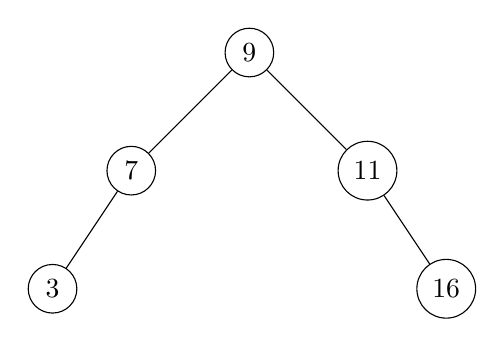
\begin{tikzpicture}[
			level distance=1.5cm,
			level 1/.style={sibling distance=3cm},
			level 2/.style={sibling distance=2cm},
			level 3/.style={sibling distance=2cm}
		]
		\node[circle,draw] {9}
		child {
				node[circle,draw] {7}
				child {node[circle,draw] {3}}
				child[missing] {}
			}
		child {
				node[circle,draw] {11}
				child[missing] {}
				child {node[circle,draw] {16}}
			};
	\end{tikzpicture}
	\caption{左旋转}
\end{figure}

\begin{figure}[H]
	\centering
	\begin{tikzpicture}[
			level distance=1.5cm,
			level 1/.style={sibling distance=3cm},
			level 2/.style={sibling distance=2cm},
			level 3/.style={sibling distance=2cm}
		]
		\node[circle,draw] {11}
		child {
				node[circle,draw] {9}
				child {
						node[circle,draw] {7}
						child {node[circle,draw] {3}}
						child[missing] {}
					}
				child[missing] {}
			}
		child {node[circle,draw] {16}};
	\end{tikzpicture}
	\caption{左旋转}
\end{figure}

\newpage